%%%%%%%%%%%%%%%%%%%%%%%%%%%%%%%%%%%%%%%%%
% Wenneker Article
% LaTeX Template
% Version 2.0 (28/2/17)
%
% This template was downloaded from:
% http://www.LaTeXTemplates.com
%
% Authors:
% Vel (vel@LaTeXTemplates.com)
% Frits Wenneker
%
% License:
% CC BY-NC-SA 3.0 (http://creativecommons.org/licenses/by-nc-sa/3.0/)
%
%%%%%%%%%%%%%%%%%%%%%%%%%%%%%%%%%%%%%%%%%

%----------------------------------------------------------------------------------------
%	PACKAGES AND OTHER DOCUMENT CONFIGURATIONS
%----------------------------------------------------------------------------------------

\documentclass[10pt, a4paper, twocolumn]{article} % 10pt font size (11 and 12 also possible), A4 paper (letterpaper for US letter) and two column layout (remove for one column)

%%%%%%%%%%%%%%%%%%%%%%%%%%%%%%%%%%%%%%%%%
% Wenneker Article
% Structure Specification File
% Version 1.0 (28/2/17)
%
% This file originates from:
% [http://www.LaTeXTemplates.com](http://www.LaTeXTemplates.com)
%
% Authors:
% Frits Wenneker
% Vel (vel@LaTeXTemplates.com)
%
% License:
% CC BY-NC-SA 3.0 ([http://creativecommons.org/licenses/by-nc-sa/3.0/](http://creativecommons.org/licenses/by-nc-sa/3.0/))
%
%%%%%%%%%%%%%%%%%%%%%%%%%%%%%%%%%%%%%%%%%

%----------------------------------------------------------------------------------------
%   PACKAGES AND OTHER DOCUMENT CONFIGURATIONS
%----------------------------------------------------------------------------------------
\usepackage{XCharter}
\usepackage{indentfirst}
\usepackage{tabularx}
\usepackage{fontspec}
\usepackage{graphicx}                     
\usepackage{booktabs}                     

% 1. Language Setup (English primary, Thai secondary)
\usepackage[thai,english]{babel} 

% 2. Font Setup
% Note: Make sure "Sarabun" or "TH Sarabun New" is installed on your OS environment
\newfontfamily\thaifont{Sarabun-Regular}[
    Path = ./ ,
    Extension = .ttf ,
    Script = Thai ,
    Scale = MatchLowercase ,
    % Adds explicit support for bold/italic if you have the files
    BoldFont = Sarabun-Bold , 
    ItalicFont = Sarabun-Italic ,
    BoldItalicFont = Sarabun-BoldItalic
]

% A handy macro to quickly switch scripts mid-sentence
\renewcommand{\textthai}[1]{{\thaifont #1}}
\babelprovide[font={rm=\thaifont}]{thai}

\usepackage[dvipsnames,svgnames]{xcolor} 

% 3. Bibliography Management Setup
\usepackage[style=authoryear, backend=biber, natbib=true]{biblatex}
\usepackage[autostyle=true]{csquotes} 

% NOTE: Removed conflicting \addbibresource from structure file. 
% Manage your .bib additions natively inside main.tex instead.

%----------------------------------------------------------------------------------------
%   MARGINS AND SPACING
%----------------------------------------------------------------------------------------
\usepackage{geometry} 
\geometry{
    top=1cm, 
    bottom=1.5cm, 
    left=2cm, 
    right=2cm, 
    includehead, 
    includefoot, 
}

\setlength{\columnsep}{7mm} 

%----------------------------------------------------------------------------------------
%   HEADERS AND FOOTERS
%----------------------------------------------------------------------------------------
\usepackage{fancyhdr} 
\pagestyle{fancy} 

\renewcommand{\headrulewidth}{0.0pt} 
\renewcommand{\footrulewidth}{0.4pt} 
\renewcommand{\sectionmark}[1]{\markboth{#1}{}} 

% Headers
\lhead{} 
\chead{\textit{\thetitle}} 
\rhead{} 

% Footers
\lfoot{} 
\cfoot{} 
\rfoot{\footnotesize Page \thepage} 

\fancypagestyle{firstpage}{ 
    \fancyhf{}
    \renewcommand{\footrulewidth}{0pt} 
}

%----------------------------------------------------------------------------------------
%   TITLE SECTION
%----------------------------------------------------------------------------------------
\newcommand{\authorstyle}[1]{{\large\usefont{OT1}{phv}{b}{n}\color{DarkRed}#1}} 
\newcommand{\institution}[1]{{\footnotesize\usefont{OT1}{phv}{m}{sl}\color{Black}#1}} 

\usepackage{titling} 
\newcommand{\HorRule}{\color{DarkGoldenrod}\rule{\linewidth}{1pt}} 

\pretitle{
    \vspace{-30pt} 
    \HorRule\vspace{10pt} 
    \fontsize{32}{36}\usefont{OT1}{phv}{b}{n}\selectfont 
    \color{DarkRed} 
}
\posttitle{\par\vskip 15pt} 
\preauthor{} 
\postauthor{ 
    \vspace{10pt} 
    \par\HorRule 
    \vspace{20pt} 
}

%----------------------------------------------------------------------------------------
%   ABSTRACT
%----------------------------------------------------------------------------------------
\usepackage{lettrine} 
\usepackage{fix-cm} 

\newcommand{\initial}[1]{ 
    \lettrine[lines=3,findent=4pt,nindent=0pt]{%
        \color{DarkGoldenrod}%
        {#1}%
    }{}%
}

\usepackage{xstring} 

\newcommand{\lettrineabstract}[1]{
    \StrLeft{#1}{1}[\firstletter] 
    \initial{\firstletter}\textbf{\StrGobbleLeft{#1}{1}} 
} % Specifies the document structure and loads requires packages

%----------------------------------------------------------------------------------------
%	ARTICLE INFORMATION
%----------------------------------------------------------------------------------------

\title{Introduction to Healthcare in the Context of Ageing Societies} % The article title

\author{
	\authorstyle{Natanon Kittimongkolsuk\textsuperscript{1}} % Authors
	\newline\newline % Space before institutions
	\textsuperscript{1}\institution{Chulabhorn International College of Medicine, Thammasat University}\\ % Institution 1
}

% Example of a one line author/institution relationship
%\author{\newauthor{John Marston} \newinstitution{Universidad Nacional Autónoma de México, Mexico City, Mexico}}

\date{\today} % Add a date here if you would like one to appear underneath the title block, use \today for the current date, leave empty for no date

%----------------------------------------------------------------------------------------

\begin{document}

\maketitle % Print the title

\thispagestyle{firstpage} % Apply the page style for the first page (no headers and footers)

%----------------------------------------------------------------------------------------
%	ABSTRACT
%----------------------------------------------------------------------------------------

\lettrineabstract{Healthcare is changing at a rapid pace: technology is evolving, and new treatements are being implemented at a breakneck pace on a global scale.
However, healthcare still reamins limited in many aspects. One critial aspect is health and wellbeing for the elderly population.
While tecnology enabling effective care for vulnerable populations has increased, many needs remain unmet. Among them are access to healthcare,
effective nutrition and food technology, availability of tools for medication management and rehabilitation, support for mental health, 
as well as community-driven care. This booklet aims to explore these topics briefly and provide a foundation to solve issues at large.}
\newline{}\emph{NOTE: This text was written as a part of the SCORE Research Camp x Hackathon 2025/26. It is intended as only a brief overview of the topic for
hackathon participants. Please perform your own research to support ideas being pitched. Furthermore, please do not limit innovations to the 
topics discussed within this document.}
%----------------------------------------------------------------------------------------
%	ARTICLE CONTENTS
%----------------------------------------------------------------------------------------
\section{Ageing Societies}
\section{Thailand's Healthcare System}
\subsection{Inequity of Healthcare}
\subsection{Pressing Challenges}

\section{Social Context}
Healthcare is more than just treating symptoms and prescribing medicines for illness. Effective healthcare demands
the involvement of medical practitioners in the community, both at the individual and community scale. Consequently,
community relationships serve as a key method for the prevention of disease and to increase the availability of healthcare
within communities, especially those in remote areas. Thailand is unique in this context, with a large network of community
healthcare practitioners known as ``village health volunteers (VHVs)'' who serve to protect the health of their communities, monitor
vulnerable residents and effectively report community health status to the relevant authorities to promote informed policy
decisions that reflect community status at both the community and country scale by narrowing the gap between policymakers
and residents of the local area. (One way to define the decentralization of healthcare is the term ``community based care'').
\\Community based care is an effective system, though it has some limitations, including the risk of decreasing equitability
of care, to the limited technology available for VHVs. Solutions to these problems are few and far between, but
could hold the potential to be highly effective and beneficial for the community at large.
\subsection{Expectations of Healthcare}
\subsection{The Mental Health Stigma}
\subsection{Healthy Habits}
One challenge to providing effective preventative healthcare for the general population is the lack of
action regarding healthy eating habits. The typical Thai meal does not cover all nutritional bases, and often
exceeds healthy levels for many macronutrients, including calories, carbohydrate, fats, salt and sugar. The habit of choosing
food that is highly flavorful and relatively in excess compared to the nutritional requirements may result in long–term
consequences such as the increased risk for NCDs, including renal, cardiovascular and diabetes related complications.
\section{Challenges for the Elderly}
\subsection{Non-communicable Diseases}
\subsection{Rehabilitation Medicine}
\subsection{Wholistic Life Quality}
\subsection{Determinants of Health}
The quality of life of a population is determined by a wide range of factors, including social environment,
region, social equitability and personal factors among others. Though over 30 years has passed, the Dahlgren and Whitehead
remains one of the standard ways of understanding the influences of health even before a visit to the medical practitioner.
Many solutions for wellbeing do not start in the hospital, but instead in the community, where interventions are often more
effective than treatment of already developed conditions. The prevention of disease, especially non–communicable diseases
remains more cost effective than treatment. However, many limitations remain that result in social interventions being overlooked.
Solutions in this field are direly needed, and may serve to actively enable the prevention of diseases in the subclinical phase,
resulting in healthier communities and longer healthspans for the population.

\begin{figure}
	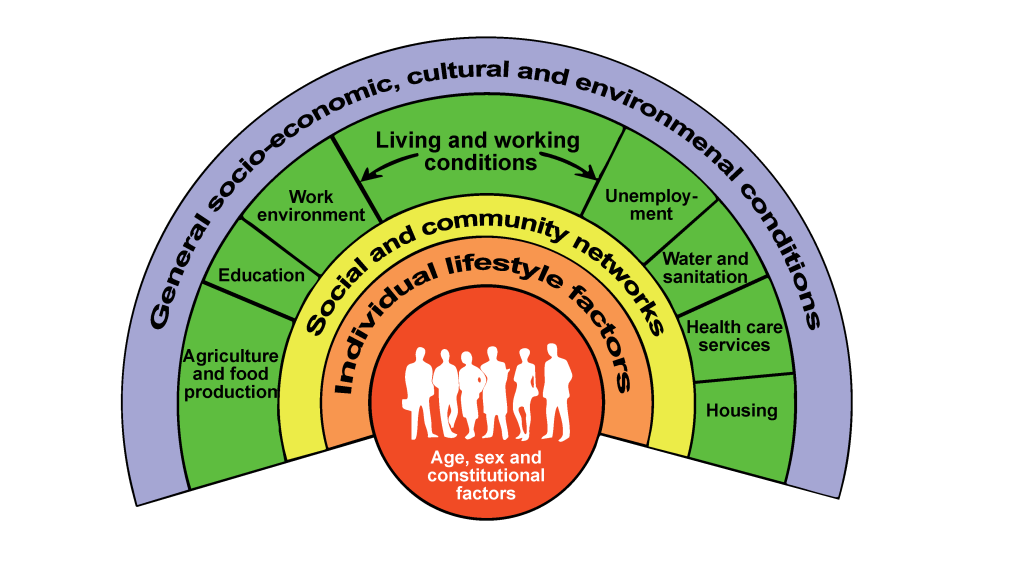
\includegraphics[width=\linewidth]{dandw.png} % Figure image
	\caption{Model of the social determinants of health (Dahlgren and Whitehead, 1991) from \cite{mariette-jb2TheoreticalModel}} % Figure caption
	\label{Dhalgren} % Label for referencing with \ref{bear}
\end{figure}

\section{Technological Advances}
\subsection{The Internet of Things}
\subsection{``The Cloud''}
\subsection{Big Data Advances}
\subsection{Artificial Inteligence}



\begin{itemize}
	\item First item in a list 
	\item Second item in a list 
	\item Third item in a list
\end{itemize}

Nunc egestas quis leo sed efficitur. Donec placerat, dui vel bibendum bibendum, tortor ligula auctor elit, aliquet pulvinar leo ante nec tellus. Praesent at vulputate libero, sit amet elementum magna. Pellentesque sodales odio eu ex interdum molestie. Suspendisse lacinia, augue quis interdum posuere, dolor ipsum euismod turpis, sed viverra nibh velit eget dolor. Curabitur consectetur tempus lacus, sit amet luctus mauris interdum vel. Curabitur vehicula convallis felis, eget mattis justo rhoncus eget. Pellentesque et semper lectus.

\begin{description}
	\item[First] This is the first item
	\item[Last] This is the last item
\end{description}

Donec nec nibh sagittis, finibus mauris quis, laoreet augue. Maecenas aliquam sem nunc, vel semper urna hendrerit nec. Pellentesque habitant morbi tristique senectus et netus et malesuada fames ac turpis egestas. Maecenas pellentesque dolor lacus, sit amet pretium felis vestibulum finibus. Duis tincidunt sapien faucibus nisi vehicula tincidunt. Donec euismod suscipit ligula a tempor. Aenean a nulla sit amet magna ullamcorper condimentum. Fusce eu velit vitae libero varius condimentum at sed dui.

%------------------------------------------------

\subsection{Subsection}

In hac habitasse platea dictumst. Etiam ac tortor fermentum, ultrices libero gravida, blandit metus. Vivamus sed convallis felis. Cras vel tortor sollicitudin, vestibulum nisi at, pretium justo. Curabitur placerat elit nunc, sed luctus ipsum auctor a. Nulla feugiat quam venenatis nulla imperdiet vulputate non faucibus lorem. Curabitur mollis diam non leo ullamcorper lacinia.

Morbi iaculis posuere arcu, ut scelerisque sem. Class aptent taciti sociosqu ad litora torquent per conubia nostra, per inceptos himenaeos. Mauris placerat urna id enim aliquet, non consequat leo imperdiet. Phasellus at nibh ut tortor hendrerit accumsan. Phasellus sollicitudin luctus sapien, feugiat facilisis risus consectetur eleifend. In quis luctus turpis. Nulla sed tellus libero. Pellentesque metus tortor, convallis at tellus quis, accumsan faucibus nulla. Fusce auctor eleifend volutpat. Maecenas vel faucibus enim. Donec venenatis congue congue. Integer sit amet quam ac est aliquam aliquet. Ut commodo justo sit amet convallis scelerisque.

\begin{enumerate}
	\item First numbered item in a list
	\item Second numbered item in a list
	\item Third numbered item in a list
\end{enumerate}

Aliquam elementum nulla at arcu finibus aliquet. Praesent congue ultrices nisl pretium posuere. Nunc vel nulla hendrerit, ultrices justo ut, ultrices sapien. Duis ut arcu at nunc pellentesque consectetur. Vestibulum eget nisl porta, ultricies orci eget, efficitur tellus. Maecenas rhoncus purus vel mauris tincidunt, et euismod nibh viverra. Mauris ultrices tellus quis ante lobortis gravida. Duis vulputate viverra erat, eu sollicitudin dui. Proin a iaculis massa. Nam at turpis in sem malesuada rhoncus. Aenean tempor risus dui, et ultrices nulla rutrum ut. Nam commodo fermentum purus, eget mattis odio fringilla at. Etiam congue et ipsum sed feugiat. Morbi euismod ut purus et tempus. Etiam est ligula, aliquam eget porttitor ut, auctor in risus. Curabitur at urna id dui lobortis pellentesque.

\begin{table}
	\caption{Example table}
	\centering
	\begin{tabular}{llr}
		\toprule
		\multicolumn{2}{c}{Name} \\
		\cmidrule(r){1-2}
		First Name & Last Name & Grade \\
		\midrule
		John & Doe & $7.5$ \\
		Richard & Miles & $5$ \\
		\bottomrule
	\end{tabular}
\end{table}

%------------------------------------------------

\section{Section}

\begin{figure}
	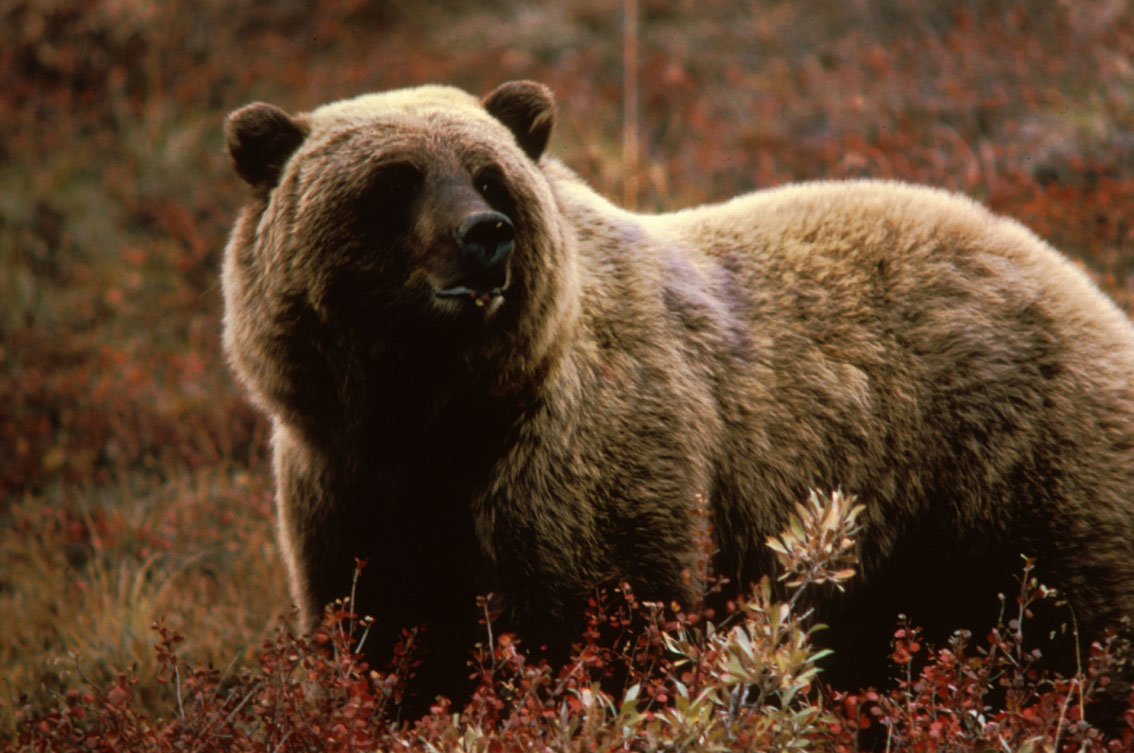
\includegraphics[width=\linewidth]{bear.jpg} % Figure image
	\caption{A majestic grizzly bear} % Figure caption
	\label{bear} % Label for referencing with \ref{bear}
\end{figure}

In hac habitasse platea dictumst. Vivamus eu finibus leo. Donec malesuada dui non sagittis auctor. Aenean condimentum eros metus. Nunc tempus id velit ut tempus. Quisque fermentum, nisl sit amet consectetur ornare, nunc leo luctus leo, vitae mattis odio augue id libero. Mauris quis lectus at ante scelerisque sollicitudin in eu nisi. Nulla elit lacus, ultricies eu erat congue, venenatis semper turpis. Ut nec venenatis velit. Mauris lacinia diam diam, ac egestas neque sodales sed. Curabitur eu diam nulla. Duis nec turpis finibus, commodo diam sed, bibendum erat. Nunc in velit ullamcorper, posuere libero a, mollis mauris. Nulla vehicula quam id tortor ornare blandit. Aenean maximus tempor orci ultrices placerat. Aenean condimentum magna vulputate erat mattis feugiat.

Quisque lacinia, purus id mattis gravida, sem enim fringilla erat, non dapibus est tellus pellentesque velit. Vivamus pretium sem quis leo placerat, at dignissim ex iaculis. Donec neque tortor, pharetra quis vestibulum id, tempus scelerisque mi. Cras in mattis est. Integer nec lorem rutrum, semper ligula bibendum, iaculis neque. Sed in nunc placerat, viverra dui in, fringilla sem. Sed quis rutrum magna, vitae pellentesque eros.

Praesent maximus mauris vitae nisl pulvinar, at tristique tortor aliquam. Etiam sit amet nunc in nulla vulputate sollicitudin. Aliquam erat volutpat. Praesent pharetra gravida cursus. Quisque vulputate lacus nunc. Integer orci ex, porttitor quis sapien id, eleifend gravida mi. Etiam efficitur justo eget nulla congue mattis. Duis commodo vel arcu a pretium. Aenean eleifend viverra nisl, nec ornare lacus rutrum in.

Vivamus pulvinar ac eros eu pellentesque. Duis nibh felis, sagittis sed lacus at, sagittis mattis nisi. Fusce ante dui, tincidunt in scelerisque ut, sagittis at magna. Fusce tincidunt felis et odio tincidunt imperdiet. Cras ut facilisis nisl. Aliquam vitae consequat metus, eget gravida augue. In imperdiet justo quis nulla venenatis accumsan. Aliquam aliquet consectetur tortor, at sollicitudin sapien porta sed. Donec efficitur mauris id rhoncus volutpat. Vestibulum ante ipsum primis in faucibus orci luctus et ultrices posuere cubilia Curae; Sed bibendum purus dapibus tincidunt euismod. Nullam malesuada ultrices lacus, ut tincidunt dolor. Etiam imperdiet quam eget elit tincidunt scelerisque. Curabitur ut ullamcorper dui. Cras gravida porta leo, ut lobortis nisl venenatis pulvinar. Proin non semper nulla.

Praesent pretium nisl purus, id mollis nibh efficitur sed. Sed sit amet urna leo. Nulla sed imperdiet sem. Donec ut diam tristique, faucibus ligula vel, varius est. In ipsum ligula, elementum vitae velit ac, viverra tincidunt enim. Phasellus gravida diam id nisl interdum maximus. Ut semper, tortor vitae congue pharetra, justo odio commodo urna, vel tempus libero ex et risus. Vivamus commodo felis non venenatis rutrum. Sed pulvinar scelerisque augue in porta. Sed maximus libero nec tellus malesuada elementum. Proin non augue posuere, pellentesque felis viverra, varius urna. Lorem ipsum dolor sit amet, consectetur adipiscing elit. Donec dignissim urna eget diam dictum, eget facilisis libero pulvinar.

Aliquam ex tellus, hendrerit sed odio sit amet, facilisis elementum enim. Suspendisse potenti. Integer molestie ac augue sit amet fermentum. Vivamus ultrices ante nulla, vitae venenatis ipsum ullamcorper sed. Phasellus gravida felis sapien, ac porta purus pharetra quis. Sed eget augue tellus. Nam vitae hendrerit arcu, id iaculis ipsum. Pellentesque sed magna tortor.

In ac tempus diam. Sed nec lobortis massa, suscipit accumsan justo. Quisque porttitor, ligula a semper euismod, urna diam dictum sem, sed maximus risus purus sit amet felis. Fusce elementum maximus nisi a mattis. Nulla vitae elit erat. Integer sit amet commodo risus, eget elementum nulla. Donec ultricies erat sit amet sem commodo iaculis. Donec euismod volutpat lacus, ut tempor est lacinia a. Vivamus auctor condimentum tincidunt. Praesent sed finibus urna. Sed pellentesque blandit magna et rhoncus.

Integer vel turpis nec tellus sodales malesuada a vel odio. Fusce et lectus eu nibh rhoncus tempus vel nec elit. Suspendisse commodo orci velit, lacinia dictum odio accumsan et. Vivamus libero dui, elementum vel nibh non, fermentum venenatis risus. Aliquam sed sapien ac orci sodales tempus a eget dui. Morbi non dictum tortor, quis tincidunt nibh. Proin ut tincidunt odio.

Pellentesque ac nisi dolor. Pellentesque maximus est arcu, eu scelerisque est rutrum vitae. Mauris ullamcorper vulputate vehicula. Praesent fermentum leo ac velit accumsan consectetur. Aliquam eleifend ex eros, ut lacinia tellus volutpat non. Pellentesque sit amet cursus diam. Maecenas elementum mattis est, in tincidunt ex pretium ac. Integer ultrices nunc rutrum, pretium sapien vitae, lobortis velit.

%----------------------------------------------------------------------------------------
%	BIBLIOGRAPHY
%----------------------------------------------------------------------------------------

\printbibliography[title={Bibliography}] % Print the bibliography, section title in curly brackets

%----------------------------------------------------------------------------------------

\end{document}
